\documentclass[]{article}

\usepackage[left=1in,right=1in,top=1in,bottom=1in]{geometry}
\usepackage{amsmath,amsfonts}
\usepackage{graphicx}
\usepackage{hw}

\setlength{\parindent}{0pt}

\graphicspath{ {.} }


\begin{document}
\section*{Q1}
1. True. The original representation can be well reconstructed based on succinct representation, while the outliers cannot be well constructed based on this method.

2. True. The diameter of a graph is the length of the shortest path between the most distanced nodes. So for a fully-connected graph, the diameter is always 1.

3. The core idea of proximity-based outlier detection is that objects that are far from others can be regarded as outliers. The proximity of an outlier object to its nearest neighbors significantly deviates from the proximity of most other objects to their nearest neighbors.

4. First, parameter sharing makes CNN computationally efficient; Second, it's translational equivalence which gives the same output for the same input at different locations; Third, CNN has sparse interactions which makes it more robust to overfitting and reduces training time. 

5. Translational equivalence means the translation of input results in an equivalent translation in the output. Translational invariance means the translation of input won't change the output at all.

6. Dropout is a kind of regularization technique. It forces the model to be more robust to noise and to learn more generalizable features.

7. $\bar{C}=\cfrac{1}{n}\sum_{i=1}^nC_i=\cfrac{1}{8}(0+\cfrac{2\times1}{3\times2}+\cfrac{2\times1}{3\times2}+\cfrac{2\times2}{3\times2}+\cfrac{2\times4}{6\times5}+1+\cfrac{2\times2}{3\times2}+1)=\cfrac{8}{15}$ 

\newpage

\section*{Q2}
\subsection*{(a)} 
Distance-based outlier detection relies on checking if there are enough objects in a sample's neighborhood. The numerator represents the number of neighbors of a sample $o$ whose distance is less than the neighborhood distance threshold $r$. The denominator means the size of the whole dataset. If their ratio is less than a given fraction threshold $\pi$, it means there are not enough neighbors ofa  sample $o$, which is an outlier.

\subsection*{(b)} 
Since $o_k$ is the k-nearest neighbor of $o$ where $k=\lceil\pi\|D\|\rceil$, if $o_k$ is the valid neighbor of a sample $o$, sample $o$ should have at least $k$ neighbors which are within the range of distance threshold. So $o$ is not an outlier in this case. However, if $dist(o,o_K)>r$, it means $o_k$ is not a valid neighbor of $o$, and $o$ is an outlier. 

\subsection*{(c)}
Considering $r=2$, point $-4.5$ has 3 neighbors, $\cfrac{3}{\|D\|}=3/10=0.3>\pi$. Not an outlier. 

Similarly, Point $-4,-3,-2.5$ has 3 neighbors with a fraction of $0.3$. Not outliers. 

Point $0$ has 0 neighbors with a fraction of $0<\pi$. It's an outlier.

Points $3, 3.5, 4, 4.5, 5$ have 4 neighbors with fraction of $0.4>\pi$. Not outliers. 

So point $0$ is the DB(2,0.2) outlier. 

\newpage

\section*{Q3}
\subsection*{(a)} Distance-based outlier detection relies on the neighborhood of a sample, which doesn't need to check the status of its neighbors. A density-based method needs to calculate the density of a sample and check against its neighboring objects. 

\subsection*{(b)} 
(i) It means the averaged smoothed distances from each neighbor $o'$ of sample $o$, where the k-nearest neighbor determines the minimum neighborhood of the sample. 

(ii) If $o$ is closer to a cluster, the distance of the k-nearest neighbor should be smaller. Then the $reachdist_k$ is smaller and $lrd_k(o)$ is larger. 

\subsection*{(c)}
(i) The numerator is the ratio of the local reachability density of sample $o$ and those of $o$'s k-nearest neighbors. In this case, if $o$ is an outlier, the local reachability density is low. 
The lower local reachability density of $o$ and the higher the local reachability densities of the k-nearest neighbors of $o$. 
If only $\sum lrd_k(o')$ is used, only the sample's neighbors are considered. It's hard to say if this density is high or low without comparison because different clusters may have various characteristics. 

(ii) To average or normalize the ratios of local reachability density between the sample and its neighbors. In this way, the result can be comparable even though the hyperparameter k is changed. 

I don't think they are comparable. If various points have the same distance as that of k-nearest neighbor. that means the $\|N_k(i)\|$ may not equal to $\|N_k(j)\|$. Those with larger number of neighbors usually have higher LOF values, even the point distributions are very close. 

\newpage
\section*{(Q4)}
\subsection*{(a)}
a: local maximal; b: saddle point; c: cliff; d: local minimal 

\subsection*{(b)}
1. Let $\sigma$ be the sigmoid function, $O_k=\delta(y)$ and y is the input of output node k,

$\delta_k=\cfrac{\partial L}{\partial y}
=\cfrac{1/2\sum(T-\sigma(y))^2}{\partial\sigma(y)}*\cfrac{\partial \sigma(y)}{\partial y}=(T-\sigma(y))(\sigma(y)(1-\sigma(y)))=O_k(1-O_k)(T-O_k)$

2. Based on the network architecture, let $x$ be the input of node $j_t$ where $x=\sigma(w_{ij} I_i)+b$ and $O_i=w_{ij} I_i$, \\
$\delta_i= \cfrac{\partial L}{\partial I_i}=\sum_j \cfrac{\partial L}{\partial x}*\cfrac{\partial x}{\partial I_i}=\sum_j \delta_j \cfrac{\sigma(w_{ij} I_i)+b}{\partial I_i}=\sum_j \delta_j w_{ij} O_i(1-O_i)=O_i(1-O_i)\sum_jw_{ij}\delta_j$

3. For L is cross-entropy, similar to 1, $\delta_k=\cfrac{\partial L}{\partial y}=\cfrac{\partial L}{\partial O_k}*\cfrac{\partial O_k}{\partial y}$, where $O_k=\sigma(y)$

Since $\cfrac{\partial{L}}{\partial O_k}=\cfrac{\partial}{\partial O_k}(-TlogO_k-(1-T)log(1-O_k))=-\cfrac{T}{O_k}+\cfrac{1-T}{1-O_k}=\cfrac{O_k-T}{(1-O)kO_k}$, then \\
$\delta_k=\cfrac{O_k-T}{(1-O)kO_k}O_k(1-O_k)=O_k-T$

4. When the loss function is MSE, the error would be close to 0 if the output unit is saturated because $O_k$ is close to 0. So little derivative can be backpropagated to cause gradient vanishing. However, if cross-entropy is used, the error can be 0 only when $O_i$ equals the target. For the sigmoid output close to 0 or 1, an error always exists so that gradient vanishing can be avoided. 


\newpage

\section*{Q5}
\subsection*{(a)}
Feature map of $K_1$: $[[0, 2, 1, 0],[1, 1, 0, 2],[2, 0, 2, 1],[1, 2, 0, 1]]$ 

Feature map of $K_2$: $[[2, 1, 1, 2],[1, 2, 1, 2],[1, 2, 1, 2],[3, 1, 1, 1]]$

\subsection*{((b))}
For the feature map convolved by kernel $K_1$, the pooled feature map is $[[1,0.75],[1.25,1]]$

For the feature map convolved by kernel $K_2$, the pooled feature map is $[[1.5,1.5],[1.75,1.25]]$

\subsection*{(c)} 
The shape of output feature map is ($\lfloor\cfrac{N-K}{S}\rfloor+1, \lfloor\cfrac{N-K}{S}\rfloor+1, L$)


\subsection*{(d)}
$h_1=Ux_1+Wh_0=\newmat{2\\2}$

$h2=Ux_2+Wh_1=\newmat{5\\3}$

$\hat{y}_2=Vh_2=\newmat{8\\5}$

\subsection*{(e)}

\begin{figure}[!ht]
    \centering
    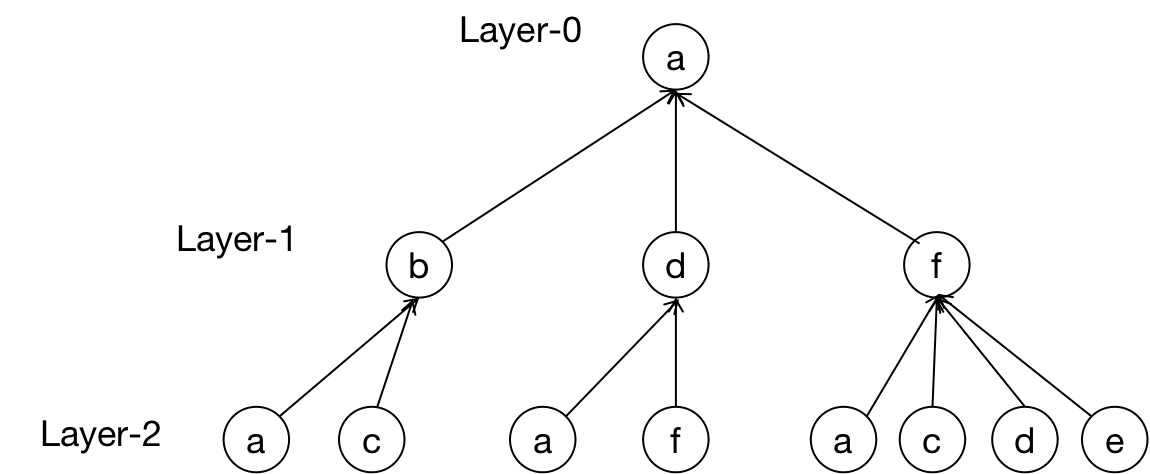
\includegraphics[width=0.8\textwidth]{fig/hw2_q5.png}
\end{figure}

\newpage

\section*{Q6}
\subsection*{(a)}
The total number of samples and features is 49534 and 27, respectively. 

\subsection*{(b)}
Mirco F1 score of LOF method is $0.90$ (See zongfan2\_HW2\_question6.py)

\subsection*{(c)}
Micro F1 score of autoencoder method is $0.878$ by setting the number neurons of hidden layers as $(27, 13, 13, 27)$ (See zongfan2\_HW2\_question6.py).

\newpage
\section*{Q7}
\subsection*{((a))}
10 classes; 5,0000 training images; 1,0000 testing images; image shape is $32\times 32\times3$

\subsection*{(b)}
ResNet50 was used as the classification network. 
Initially, the training had 200 epochs. But the loss seemed to not converge. Then the trained model weights were loaded and retrained for another 300 epochs.

\begin{figure}[!ht]
    \centering
    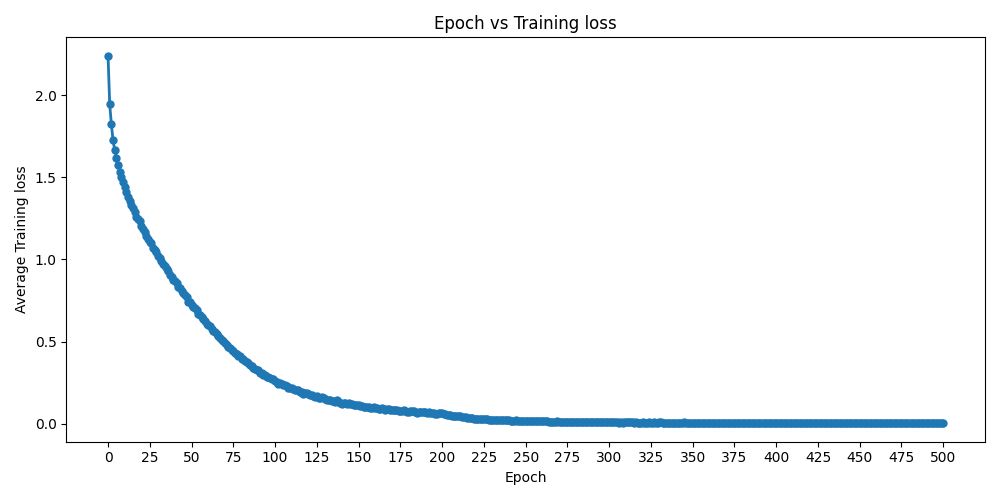
\includegraphics[width=0.8\textwidth]{fig/hw2_q7.png}
\end{figure}


\subsection*{(c)}
The final accuracy is $84.15\%$ (see zongfan2\_HW2\_question7.py file)


\newpage

\section*{Q8}

\subsection*{(a)}
This is because the first eigenvalue of the adjacency matrix is the largest eigenvalue. Intuitively, the larger the largest eigenvalue is, the more connected the graph is, and therefore the more vulnerable the graph structure is under epidemic.

\subsection*{(b)}

1. The first-eigenvalue based vulnerability score is not necessarily comparable between graphs with a different number of nodes. If two graphs with the same vulnerability score but a different number of nodes, this does not necessarily mean that they two have the same ability to contain the epidemic. 

2. When the adjacency matrix is extremely large, computing the first eigenvalue might be computationally intractable. 


\subsection*{(c)}
The goal of shield score is to quantify the importance of a given set of nodes S, and specifically the impact of their deletion/immunization to the vulnerability of the rest of the graph. The obvious choice is the drop in eigenvalue that their removal will cause to the graph.
The shield value is defined as $Sv(S)=\sum_{i\in S}2\lambda u(i)^2-\sum_{i,j\in S}A(i,j)u(i)u(j)$.
Intuitively, a set of nodes S has higher shield value score if (1) each of them has a high eigen-score $u(i)$,
and (2) they are dissimilar with each other (small or zero
A(i,j)).
In addition, shield value is monotonically non-decreasing, which can find the near-optimal solution using greedy approach and improve improve computation efficiency.

\subsection*{(d)}
1. Time complexity of NetShield is $O(nk^2+m)$, where n is the number of nodes and m is the number of edges in the graph S, and k is the number of nodes in the subgraph of S. 

NetShield algorithm's first step is to calculate the first eigenvalue, which costs $O(m)$. Next, calculating the shield score of each individual node costs $O(n)$.
Then greedily selecting one more node and adding it into set S costs $O(n)+O(n*iter)$. So the overall computational cost is $O(m)+O(n)+\sum_{iter=1}^k(n+n*iter)=O(nk^2+m)$

2. Space comparable is $O(n+m+k)$. The space cost of the first step to calculate eigenvalue is $O(n+m+1)$, where $O(n+m)$ is used to run the eigendecomposition algorithm, $O(n)$ is to store u and $O(1)$ is to store $\lambda$. 
The cost to initialize S is $O(1)$. The cost to calculate the shield score for each node is an additional $O(n)$ space. Then, it takes $O(n)$ space for each inner loop to find a node to be added into S. This space can be re-used for the next iteration until all k nodes are iterated. The selected nodes need $O(k)$. So the overall space cost is $O(n+m+k)$

\subsection*{(f)}
For the NetShield algorithm, there is a limitation on the number of nodes to immunize in order to get a good approximation of $\Delta\lambda(S)$ with shield score $S_r(S)$, which might not hold when the max degree of the graph is relatively small.
$NetShield+$ algorithm is proposed to solve this problem by finding out k nodes iteratively rather than finding out all the k nodes to delete in one round as in
NetShield. By fixing a batch number $b$, $NetShield+$ would pick out and delete b best nodes for the current graph at each round, and then use the updated graph for the next round of computation. 

The advantages of $NetShield+$ also include improved time efficiency with a complexity of $O(mk/b+nkb)$. This linear property makes it better for larger size of input graph. 

\newpage

\section*{(Q9)}

\subsection*{((a))}
$1-(1-\beta)^n$

\subsection*{(b)}
The largest eigenvalue is 38.6

\subsection*{(c)}
\begin{figure}[!ht]
    \centering
    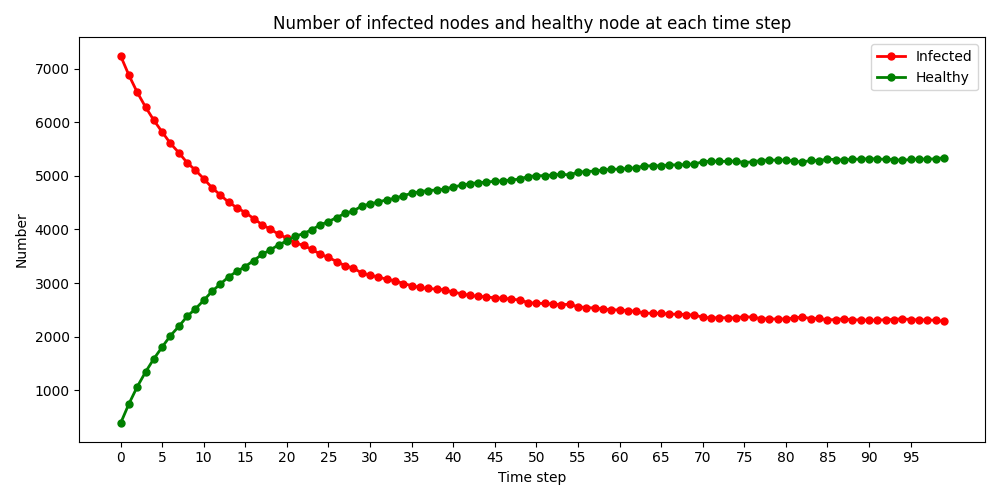
\includegraphics[width=0.8\textwidth]{fig/hw2_q9_c.png}
\end{figure}

$\cfrac{\beta\lambda}{\delta} = 7.72>1$. The epidemic won't stop. This result aligns with the theory. 

\subsection*{(d)}
\begin{figure}[!ht]
    \centering
    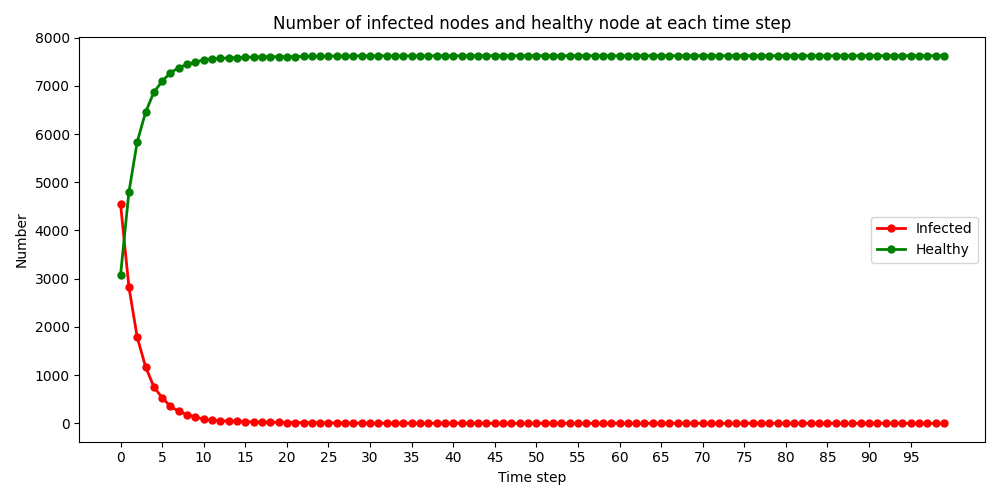
\includegraphics[width=0.8\textwidth]{fig/hw2_q9_d.png}
\end{figure}

$\cfrac{\beta\lambda}{\delta} = 0.965<1$. The epidemic stops. This result aligns with the theory. 

The code can be found in "zongfan2\_HW2\_question9.py"

\end{document}